
\begin{figure}[h]
  \centering
  \begin{tabular}{  c p{0.7cm} c}
    %\centering
    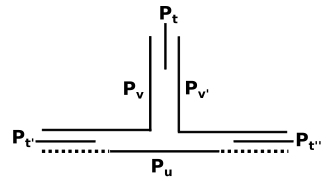
\includegraphics[width=5.5cm]{img/clawGrid} & &
    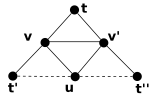
\includegraphics[width=3.5cm]{img/clawInduced.png}
    \\
    \footnotesize %\centering 
    (a)  \footnotesize Clique-garra com caminhos adicionais. && \footnotesize (b) Subgrafo induzido pelos caminhos.\\
  \end{tabular}

 \caption{Reconstrução do modelo de intersecção.}
 \label{fig:clawGrid}
\end{figure} 

 
